% !TEX root = ./main.tex
\chapter{Modeling tools}
This chapter discusses the modeling tools necessary for conducting simulations presented in this thesis. A description of the transport treatment, large-eddy simulations, is provided alongside discussion of requisite sub-grid scale parameterizations that we utilize. Attributes of the computational domain, including its spatial extent, grid resolution, and other defining qualities are presented. Meteorological initial conditions for simulations are discussed as well as determination of necessary spin-up time for the development of convective boundary layer in the computational domain. Subsequently, chemical mechanisms used for gas phase and aerosol chemistry are discussed. Lastly, the aerosol model, PartMC, and its coupling with the chosen transport model is discussed. 

\section{Large-eddy simulations}
Within the planetary boundary layer (PBL), turbulent eddies are responsible for mixing and transporting gases and aerosol particles as well as thermal and kinetic energy. Over time, these eddies break down due to flow instabilities, frictional losses due to interactions with physical boundaries, and the viscosity of the atmospheric constitutents. Therefore, it is important for modeling frameworks that represent the PBL to explicitly resolve the physical scales over which transport and mixing occur, as well as accurately model the dynamical tendency of kinetic energy transfer from large to small eddies. 

Representation of turbulence in modeling frameworks is a computationally challenging task because of the range of scales one must consider and the associated need for high spatial resolution. In the PBL, turbulent eddies range in size from hundreds of meters (\hl{check this}) to the Kolmogorov length scale on the order of 1 mm (\hl{check this, cite Kolmogorov et al. 1991}), at which size eddies break down due to kinematic viscosity of atmospheric constituents.\hl{could talk about DNS here} A widespread technique when modeling the PBL is the use of large-eddy simulations (LES). \hl{Could discuss and include citations to fundamental papers like Smagorinsky, Deardorff, etc.} In LES, the equations of motion are filtered such that the largest, energy-containing eddies are explicitly resolved down to a grid resolution on the order of 10 meters. For eddies smaller than the resolution of the grid, sub-grid scale (SGS) parameterizations are used to represent the statistical attributes of unresolved eddies, including their energy dissipation and stress forces.  

For simulation results presented in this thesis, we use the Weather Research and Forecasting model (WRF) configured for LES \hl{cite WRF}. In practice, conducting LES studies in WRF arises from modeling choices including the representation of SGS turbulence parameterizations and adequately high grid resolution; that is, there is no ``switch" for configuring WRF in LES mode, but rather structural choices which permit representation of the relevant dynamics. 

\subsection{Sub-grid scale parameterizations}
A key choice in the implementation of LES is the selection of SGS turbulence parameterizations. Specifically, one must parameterize the SGS stress $\tau_{ij}$ and SGS flux $q_i$. The stress tensor $\tau_{ij}$ represents the deformational forces acting both normal ($i=j$) and perpendicular ($i\neq j$) to each grid cell, while the SGS flux $q_i$ refers to the transport of scalars such as momentum, heat, or other quantities by unresolved eddies. A common technique for the closure of SGS stress and flux is the use of eddy-viscosity models. This technique was pioneered by Smagorinsky for parameterizing the motion of SGS eddies in a model of general circulation (\cite{smagorinsky_general_1963}). Eddy-viscosity models mimic the linear relationship between the stress tensor of a Newtonian fluid and shearing forces acting on the fluid scaled by the fluid's molecular viscosity. As such, eddy-viscosity models are not fundamentally grounded in physical tendencies of turbulent flows, but rather provide an empirical approximation that mimics Newtonian fluids and has been shown to be reasonable for representing SGS turbulence in modeling studies of the PBL \hl{cite?}. The SGS stress and SGS flux are then expressed as 
\begin{align}
\tau_{ij} &= -2\nu_T \tilde{S}_{ij},\\
q_i &= -\nu_{\theta}\frac{\partial \tilde{\theta}}{\partial x_i}, 
\end{align}
where $\nu_T$ is the eddy viscosity coefficient, $\tilde{S}_{ij} = \frac{1}{2} (\partial\tilde{u_i}/\partial x_j + \partial\tilde{u_j}/\partial x_i )$ is the resolved strain rate tensor (i.e., the rate at which straining forces such as expansion and shearing due to resolved flow occur), $\nu_{\theta}$ is the eddy diffusivity coefficient for some scalar quantity $\theta$, and $\partial \tilde{\theta} / \partial x_i$ is the resolved-scale gradient of scalar $\theta$ in direction $x_i$. As $\tilde{S}_{ij}$ and $\partial \tilde{\theta} / \partial x_i$ are known quantities determined at the resolved scale, eddy-diffusivity models then become a matter of determining $\nu_T$ and $\nu_{\theta}$. 

\hl{Note to self, use Stoll in here somewhere?}
(\cite{stoll_large-eddy_2020})

Deardorff was the first to implement Smagorinsky's eddy-diffusivity SGS model for LES, however, he found that the model was overly diffusive for short wavelength features (\cite{deardorff_numerical_1970}). \cite{deardorff_stratocumulus-capped_1980} instead proposed an alternative eddy-diffusivity model in which a prognostic equation for SGS kinetic energy $E$ is solved alongside expressions for $\nu_T$ and $\nu_{\theta}$
\begin{align}
\frac{\partial E}{\partial t}  &= -\frac{\partial\tilde{u_j}E}{\partial x_j} + 2\nu_T\tilde{S}_{ij}\tilde{S}_{ij} - \nu_{\theta}\frac{\partial \tilde{b}}{\partial z} + \frac{\partial}{\partial x_j}2\nu_T\frac{\partial E}{\partial x_j} - \epsilon, \\
\nu_T &= C_1\ell\sqrt{E}, \\ 
\nu_{\theta} &= \left(1 + 2 \frac{\ell}{\Delta}\right)\nu_T,
\end{align}
where $b$ is buoyancy, $\epsilon$ is the turbulent kinetic energy (TKE) dissipation, $C_1$ is a coefficient that must be specified by the modeler, and $\ell$ is the turbulent length scale. Customarily, $C_1 = 0.1$ and we use this value as recommended by an idealized test case for LES simulations packaged alongside the WRF codebase.

% Some stuff about Smagorinsky's eddy diffusivity model that I don't think pertains to my simulations
\iffalse

Smagorinksy showed that the SGS stress can be represented as the following 
\begin{equation}
	\tau_{ij} = -2\left(C_S\Delta\right)^2 |\tilde{S}| \tilde{S}_{ij},
\label{equation:smagorinsky_sgs_stress}
\end{equation}
where $C_S$ is the Smagorinsky constant that must be specified by the modeler, $\Delta = (\Delta_x \Delta_y \Delta_z)^{1/3}$ is the geometric mean length scale for spatial discretization in a 3D domain, $|\tilde{S}| =\sqrt{2\tilde{S}_{ij}\tilde{S}_{ij}}$ is the magnitude of the resolved strain rate, and $\tilde{S}_{ij} = \frac{1}{2} (\partial\tilde{u_i}/\partial x_j + \partial\tilde{u_j}/\partial x_i )$ is the resolved strain rate tensor (i.e., the rate at which straining forces such as expansion and shearing due to resolved flow occur). The Smagorinsky constant takes values typically in the range of 0.10--0.20. In WRF-LES, we use a value of $C_S = 0.18$ as recommended by an idealized test case for LES simulations packaged alongside the WRF codebase.
\begin{table}[h!]
\centering
\begin{tabular}{||c c||} 
 \hline
 SGS Parameter & Value\\ [0.5ex] 
 \hline\hline
 $C_s$ & 0.18 \\ 
 $C_k$ & 0.1 \\ [1ex] 
 \hline
\end{tabular}
\caption{Table with SGS eddy coefficients}
\label{table:1}
\end{table}

\fi


\subsection{Computational domain}
We model the PBL in an 3D idealized domain with dimensions 10 km in both lateral dimensions and 2 km vertically. A horizontal resolution of 100 m was chosen alongside a vertical resolution of approximately 20 m\footnote{WRF uses a terrain-following pressure ``eta" coordinate system for vertical levels. Note that because the domain only extends to 2 km vertically, vertical levels are nearly equally spaced apart.}, resulting in a domain of 100x100x100 grid cells. This resolution is necessary to resolve eddies responsible for turbulent transport in the PBL. A higher resolution vertically is desired in order to accurately represent vertical motions due to convective and turbulent transport. Time discretization is set to 1 second for all simulations, however sub-models such as chemistry (when active) further refine time discretization to maintain stability for integration. 

The domain is absent of any topographic features with a uniform, flat surface \hl{what about surface roughness, etc?}.  Latitude and Longitude coordinates of (0, 0) are used internally for computing the solar zenith angle necessary for photolysis calculations, however, the domain's idealized topography is not intended to match the geographic region surrounding these coordinates. 


\subsection{Meteorological Initial Conditions}
 
 \begin{figure}[h]
	\centering
	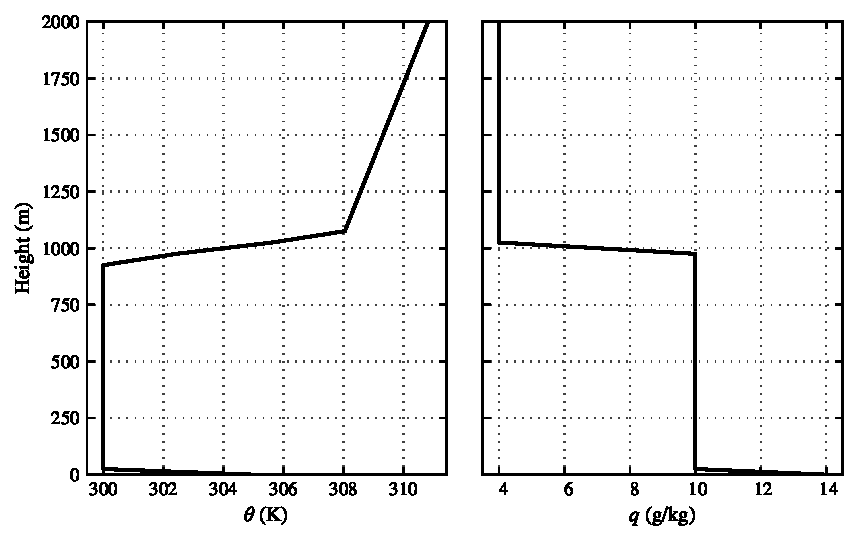
\includegraphics[width=\textwidth]{WRF-LES_default_sounding.pdf}
	\caption{Idealized atmospheric sounding used for domain meteorological initial conditions. Initial conditions for potential temperature (left) and specific humidity (right). \hl{TODO: check what is best, units in brackets or in paretheses? Figure 3.2 uses brackets so I should be consistent either way...}}
	\label{fig:sounding}
\end{figure}

The domain meteorological conditions are initialized using an ideal sounding typical of a convective boundary layer (see Figure \ref{fig:sounding}). The lowest 25 m of the atmosphere are initially unstable to allow for parcels to rise due to buoyancy into the neutral PBL that extends to approximately 1 km. Above this point, the PBL is capped by an inversion up to 2 km. 

Both zonal ($u$) and meridional ($v$) wind are set to zero throughout the entire domain. \cite{tian_how_2022} and \cite{fast_impact_2019} both show that the impact of surface heterogeneities in surface heat fluxes on cloud formation and type are sensitive to wind conditions, and are most pronounced for minimal background winds. Extending the relevance of these findings to this thesis, our choice of an initial condition characterized by zero winds is intended to isolate the impact of emissions spatial heterogeneity on the evolving atmospheric state of gasses and aerosols.

At the surface, the specific humidity $q$ is highest at 14 \si{g.kg^{-1}} and lowers to a uniform 10 g/kg within the PBL. Above the PBL, $q$ is a uniform 4 \si{g.kg^{-1}} extending vertically to the top of the domain. \hl{could also include plot of temperature and RH?}. At the surface, a uniform surface heat flux (\hl{I assume sensible?}) of 0.24 \si{K.ms^{-1}} is set and random perturbations of the temperature field are imposed at the lowest four levels to initiate turbulence. The surface heat flux is responsible for maintaining convection and turbulent transport over the course of the simulation. Boundary conditions are periodic along all lateral boundaries.

\iffalse
\begin{itemize}
\item Note the Coriolis parameter is 1e-4 which is roughly what it is at around 45 degrees lat.. this is different than the 0,0 I assume for the SZA calculations - is this passed as a value or is this calculated in the ideal initialization routine? \hl{this may actually be okay since the initial wind field is zero everywhere and turbulence and convection are the only sources of transport. The domain is also relatively small so my hunch is that the Coriolis force is insignificant. Technically I think this depends on a scale analysis using Rossby number U/lf where f is 1e-4 and U and l are the characteristic length scales for velocity and space respectively.}
\end{itemize}
\fi


\subsection{Simulation spin-up}

\begin{figure}[h]
	\centering
	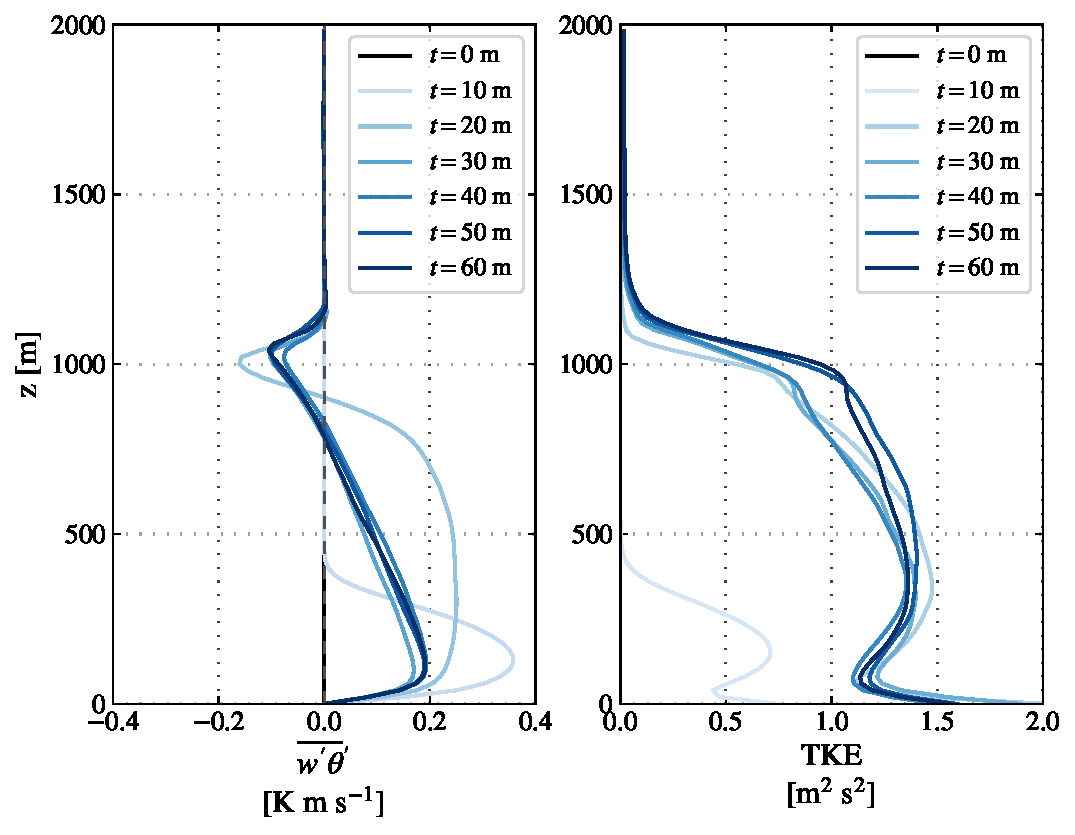
\includegraphics[width=\textwidth]{heat-flux-and-tke-profile.pdf}
	\caption{Resolved-scale vertical heat flux profiles (left) and TKE at intervals of 10 minutes during the first hour of simulation spin-up.}
	\label{fig:heat-flux}
\end{figure}

Prior to the release of gas and aerosol emissions, the simulation is allowed to spin up for a period of 1 hour. During this time, convection and turbulence within the boundary become well established and throughly mix the initial conditions for gases and aerosols alongside transporting heat and momentum. In a well established convective boundary layer, the profile of vertical heat flux should decrease approximately linearly with height. Both resolved-scale\footnote{Ideally, one would evaluate total (resolved + parameterized) vertical heat flux and total TKE. WRF does not provide output for SGS quantities, so it would be necessary for one to modify the codebase to allow exporting these additional data.} vertical heat flux and TKE profiles are shown in Figure \ref{fig:heat-flux} in increments of 10 minutes from $t=0$ minutes to $t=1$ hour. Initially, vertical heat flux is zero everywhere due to the initial condition of zero vertical velocity. At $t=10$ minutes, vertical heat flux is localized near the surface and exceeds 0.3 \si{K.m.s^{-1}}. By $t=30$ minutes, initial transient behavior in vertical heat flux relaxes as the convective boundary layer becomes more well established and the heat flux profile takes on a linearly decreasing trend with height. Profiles for subsequent times agree closely with the profile at $t=30$ minutes, indicating that the convective boundary layer is near fully established by 30 minutes. Note that the TKE profiles in Figure  \ref{fig:heat-flux} indicate that energy-containing eddies in the upper boundary layer continue to develop through $t=1$ hour, as TKE increases in the upper boundary layer from $\sim 0.7$ \si{m^2.s^2} at $t=30$ minutes to $\sim 1.1$ \si{m^2.s^2} by $t=1$ hour. Thus 1 hour of model spin-up time was chosen to adequately allow for development of the convective boundary layer and resolved scales of turbulence.


\section{Gas phase simulations}

\subsection{Chemical mechanism}
In Chapter 4, we conduct simulations with only gas phase initial conditions and emissions to isolate the impact of emissions spatial heterogeneity on gas phase reactions. For these simulations, we use WRF version 4.4.1. Beginning with WRF version 4, various sub-models including chemical mechanisms are packaged alongside the WRF codebase. We select the chemical mechanism Carbon-Bond Mechanism-Z (CBMZ) for gas phase photochemical reactions (\cite{zaveri_new_1999}). CBMZ models both inorganic and organic compounds prevalent in anthropogenic and biogenic emissions. CBMZ allows computationally efficient calculation of over 100 reactions across dozens of chemical species. This is possible due to the model's ``lumped-structure" approach to sorting similar organic compounds by their carbon bond structure (e.g, alkanes, carbonyls, etc.). This reduces the need for tracking large volumes of organic species and reactions. Despite simplifications to the organic chemistry mechanism, CBMZ has been shown to accurately represent concentrations of compounds of primary interest for atmospheric chemistry applications (e.g., O$_3$, NO$_x$, etc.) (\cite{zaveri_new_1999}, \hl{other citations?}). 

\subsection{Initial conditions and emissions}\label{gas-phase-ics-and-emiss}

\begin{table}[h]
\centering
\caption{Gas phase emissions and initial conditions. Table taken from \cite{riemer_simulating_2009} \hl{with permission}.}
\begin{tabular*}{\linewidth}{@{\extracolsep{\fill}} lccr}
\\[-2ex]\hline 
     \hline \\[-2ex] Species & Symbol & Initial Mole Fraction (ppb) & Emissions (nmol m\textsuperscript{-2} s\textsuperscript{-1}) \\
\midrule
Nitric oxide & NO & 0.1 & 31.8 \\
Nitrogen dioxide & NO\textsubscript{2} & 1.0 & 1.67 \\
Nitric acid & HNO\textsubscript{3} & 1.0 & \\
Ozone & O\textsubscript{3} & 50.0 & \\
Hydrogen peroxide & H\textsubscript{2}O\textsubscript{2} & 1.1 & \\
Carbon monoxide & CO & 21 & 291.3 \\
Sulfur dioxide & SO\textsubscript{2} & 0.8 & 2.51 \\
Ammonia & NH\textsubscript{3} & 0.5 & 6.11 \\
Hydrogen chloride & HCl & 0.7 & \\
Methane & CH\textsubscript{4} & 2200 & \\
Ethane & C\textsubscript{2}H\textsubscript{6} & 1.0 & \\
Formaldehyde & HCHO & 1.2 & 1.68 \\
Methanol & CH\textsubscript{3}OH & 0.12 & 0.28 \\
Methyl hydrogen peroxide & CH\textsubscript{3}OOH & 0.5 & \\
Acetaldehyde & ALD2 & 1.0 & 0.68 \\
Paraffin carbon & PAR & 2.0 & 96 \\
Acetone & AONE & 1.0 & 1.23 \\
Ethene & ETH & 0.2 & 7.2 \\
Terminal olefin carbons & OLET & 2.3 \(\cdot 10^{-2}\) & 2.42 \\
Internal olefin carbons & OLEI & 3.1 \(\cdot 10^{-4}\) & 2.42 \\
Toluene & TOL & 0.1 & 4.04 \\
Xylene & XYL & 0.1 & 2.41 \\
Lumped organic nitrate & ONIT & 0.1 & \\
Peroxyacetyl nitrate & PAN & 0.8 & \\
Higher organic acid & RCOOH & 0.2 & \\
Higher organic peroxide & ROOH & 2.5 \(\cdot 10^{-2}\) & \\
Isoprene & ISOP & 0.5 & 0.23 \\
Alcohols & ANOL & & 3.45 \\
\\[-2ex]\hline 
     \hline \\[-2ex]
\end{tabular*}
\label{table:gas_emiss_ics}
\end{table}

Gas phase initial conditions and emissions are chosen to represent species and concentrations typical of an urban plume and are adopted from \cite{riemer_simulating_2009}. The authors determined gas phase concentrations and emission rates via the 1987 Southern California Air Quality Study (SCAQS) data set which contains measurements of both gas phase species and particulate matter mass concentrations collected at multiple sites across the Los Angeles basin (\cite{zaveri_model_2008}). Table \ref{table:gas_emiss_ics} contains all gas phase initial conditions and emission rates \hl{Note if I didnt end up using some of these species then remove those}. Empty entries signify zero concentrations or emission rates. To allow for simulation spin-up, all emission rates are set zero during the first hour of simulations. Subsequently, emitted compounds are released only at the surface and at a constant rate as specified in Table \ref{table:gas_emiss_ics} for the remainder of the simulation.



\section{Multiphase simulations}
\subsection{Chemical mechanism}
Chapter 5 presents simulation results where both gas phase chemistry and aerosol processes (e.g., coagulation, gas-particle partitioning, etc.) are modeled. Both gas phase and aerosol chemistry is represented using the Model for Simulating Aerosol Interactions and Chemistry (MOSAIC) (\cite{zaveri_model_2008}). MOSAIC was developed by the authors of CBMZ, and it should be noted that CBMZ is included a sub-model within MOSAIC for handling gas phase chemistry. For aerosol chemistry, MOSAIC simulates dynamic gas-particle partitioning and phase-dependent thermodynamic equilibrium. A key challenge for modeling aerosol chemistry is that the coupled system of solid-liquid phase reactions that govern aerosol thermodynamic equilibrium is often numerically stiff due to the rate of reactions varying over large timescales. Often, chemical mechanisms solve such stiff systems in a computationally expensive manner either by iterative techniques or by directly minimizing the Gibbs Free energy of the system. MOSAIC takes an alternative approach whereby the system of equilibrium reactions is reformulated as a pseudo-transient system. This recasts the system as ordinary differential equations, for which standard numerical techniques are used to integrate and obtain equilibrium steady state solutions. This approach makes MOSAIC computationally efficient while maintaining good agreement when benchmarked against numerically rigorous and accurate models (\cite{zaveri_model_2008}).


\subsection{Aerosol representation}

We use the Particle Monte Carlo (PartMC) model for particle-resolved representation of aerosols (\cite{riemer_simulating_2009}). In PartMC, aerosol particles are represented via a set of computational particles with appropriate multiplicity to represent the desired aerosol population. Each computational particle is allowed to compositionally vary due to aerosol processes (e.g., coagulation, condensation, gas-particle partitioning, etc.), thus allowing the representation of a far greater degree of compositional diversity and aerosol properties than sectional or modal based aerosol models \hl{citations}. PartMC is a box model, meaning that within computational grid cells, the position of computational particles is not tracked. Instead, processes such as coagulation are handled in the probabilistic manner of \hl{Gillepsi 1975}. PartMC is coupled with MOSAIC, thereby leveraging the computational efficiency and accuracy of each model in allowing full representation of an aerosol state (number and mass concentration, per-particle composition) under aging due to both aerosol physical processes and chemical reactions.

\cite{curtis_single-column_2017} coupled PartMC-MOSAIC with WRF for a single column model of the planetary boundary layer. The authors developed approaches for modeling the turbulent diffusion and dry deposition of aerosol particles as stochastic processes. The resulting modeling framework, WRF-PartMC-MOSAIC, is extended here for use with 3D LES. 

For WRF-PartMC-MOSAIC-LES, we use 100 computational particles per grid cell for a total of 100 million computational particles throughout the domain at initialization. This value was chosen to balance computational efficiency and storage demands alongside numerical representability -- too few computational particles will result in random noise for aerosol population properties due to the stochastic nature of the PartMC model.

\subsection{Initial conditions and emissions}

Initial conditions and emissions of gas phase species match those discussed in Section \ref{gas-phase-ics-and-emiss} and displayed in Table \ref{table:gas_emiss_ics}. Similarly, aerosol initial conditions and emission rates are adopted from \cite{riemer_simulating_2009}, who based aerosol distributions, composition, and emission rates off measurements collected as part of the SCAQS campaign in the Los Angeles valley. Aerosol initial conditions and emission properties are summarized in Table \ref{table:aero_emiss_ics}. Size distributions for aerosol initial conditions and emissions are shown in Figure \ref{fig:aero_ic_dist} and Figure \ref{fig:aero_emiss_dist}, respectively. The aerosol initial condition is comprised of two modes, including a Aitken mode and accumulation mode. Each mode is an equal mixture of 50\% ammonium sulfate and 50\% primary organic aerosol (POA). Three emission modes are chosen to represent emissions from various urban combustion sources, including cooking, diesel vehicles, and gasoline vehicles. The cooking emission mode is comprised of 100\% POA and the diesel and gasoline modes are each a mixture of POA and black carbon (BC). 

\begin{table}[h]
\centering
\caption{Aerosol emissions and initial conditions. Table taken from \cite{riemer_simulating_2009} \hl{with permission}.}
\begin{tabular*}{\linewidth}{@{\extracolsep{\fill}} cccccc}
\\[-2ex]\hline 
     \hline \\[-2ex] Initial/Background  & $N$ (m$^{-3}$) & $D_{\text{gn}}$ ($\mu$m) & $\sigma_g$ & Composition by Mass\\
 \midrule
Aitken Mode & $3.2 \cdot 10^9$ & 0.02 & 1.45 & 50\% (NH$_4$)$_2$SO$_4$, 50\% POA\\
Accumulation Mode & $2.9 \cdot 10^9$ & 0.116 & 1.65 & 50\% (NH$_4$)$_2$SO$_4$, 50\% POA\\
\midrule
Emissions & $E$ (m$^{-2}$ s$^{-1}$) & $D_{\text{gn}}$ ($\mu$m) & $\sigma_g$ & Composition by Mass\\
\midrule
Meat cooking & $9 \cdot 10^6$ & 0.086 & 1.9 & 100\% POA\\
Diesel vehicles & $1.6 \cdot 10^8$ & 0.05 & 1.7 & 30\% POA, 70\% BC \\
Gasoline vehicles & $5 \cdot 10^7$ & 0.05 & 1.7 & 80\% POA, 20\% BC \\
\\[-2ex]\hline 
     \hline \\[-2ex]
\end{tabular*}
\label{table:aero_emiss_ics}
\end{table}

\begin{figure}[h]
  \centering
  \begin{subfigure}
    \centering
    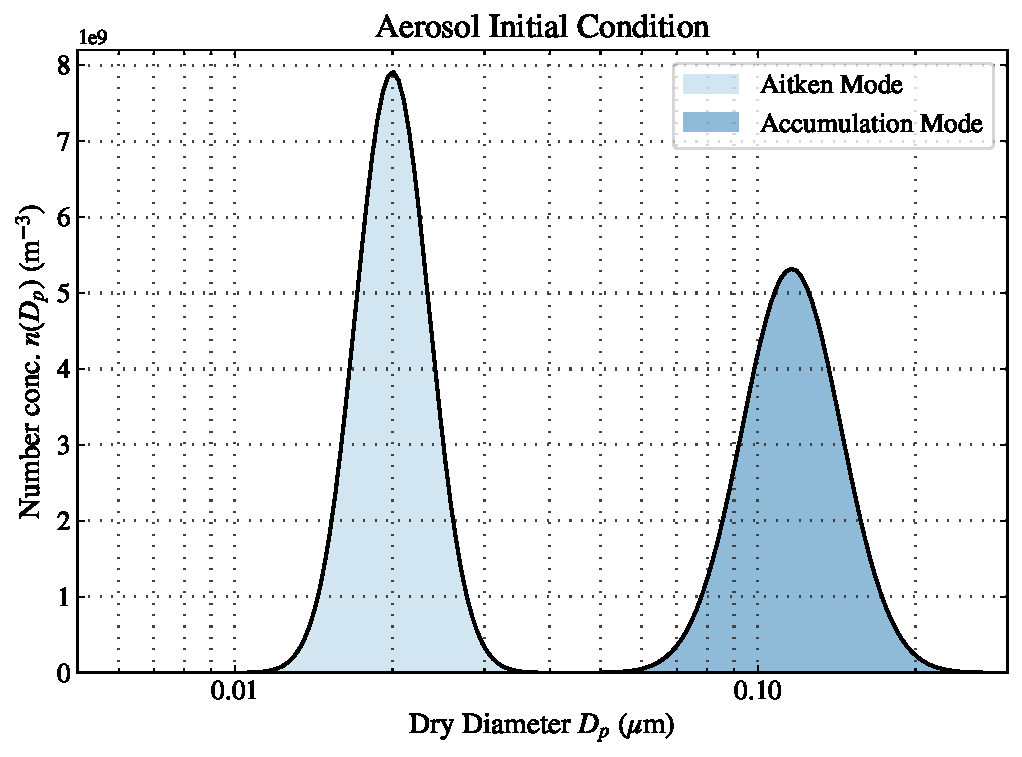
\includegraphics[width=.85\textwidth]{figures/urban-plume-aerosol-ic.pdf}
    \caption{Aerosol initial condition size distributions.}
    \label{fig:aero_ic_dist}
  \end{subfigure}
   \vspace*{5mm} 
  \begin{subfigure}
    \centering
    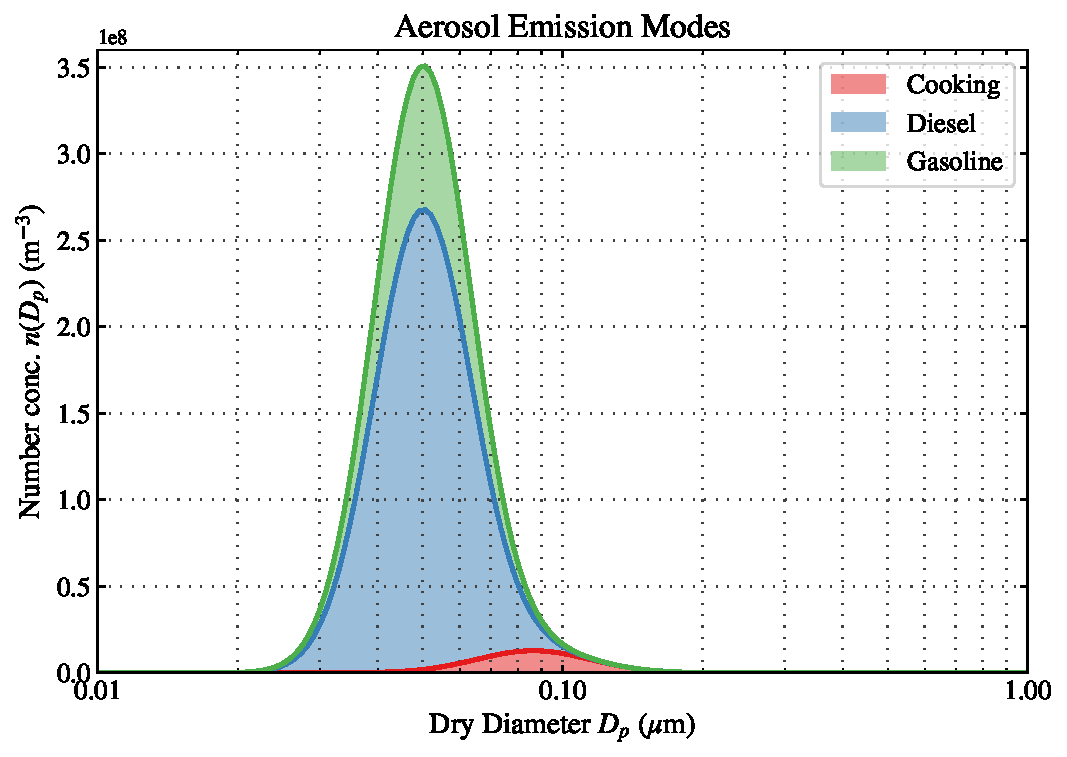
\includegraphics[width=.85\textwidth]{figures/urban-plume-aerosol-emissions.pdf}
    \caption{Aerosol emission size distributions.}
    \label{fig:aero_emiss_dist}
  \end{subfigure}
\end{figure}



